\section*{Maximum flow problem with minimum capacities}

We describe how to find the maximum flow from $S'$ to $T'$ when the edges also constrain the minimum bound of the flow amount (edges have ``minimum capacities''). It can be boiled down to an ordinary max-flow problem.

Consider an edge from $u$ to $v$ whose capacity is $R$ and minimum capacity is $L$. To deal with the minimum capacity, create a new vertex $S'$ to $T'$, remove the original edge, and add edges with the following capacities:

\begin{figure}[h]
    \centering
    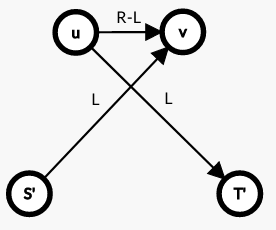
\includegraphics[width=0.5\textwidth]{flow.png}
    \caption{Flow network example with minimum capacities}
\end{figure}

Add such edges for all edges with the minimum capacities. On the resulting graph, accumulate maximum flow in the following order:

\begin{itemize}
    \item from $S'$ to $T'$
    \item from $S'$ to $T$
    \item from $S$ to $T'$
    \item from $S$ to $T$
\end{itemize}

An $S$--$T$ flow that satisfies the minimum capacities exists if and only if, for all outgoing edges from $S'$ and incoming edges to $T'$, the flow and capacity are equal. (This can be understood by corresponding the flows from $S'$ and $T'$ to the original edges.)

Alternatively, if you just want to know the existence of a flow satisfying the minimum capacities, one can add an edge from $T'$ to $S'$ with infinite capacity and consider the flow from $S'$ to $T'$ once, instead of accumulating flows four times.
